% Copyright (C) 2021 Diogo Rodrigues, Rafael Ribeiro, Bernardo Ferreira
% Distributed under the terms of the GNU General Public License, version 3

\documentclass{beamer}
% Encodings (to render letters with diacritics and special characters)
\usepackage[utf8]{inputenc}
% Language
\usepackage[english]{babel}
\usepackage{verbatim}

\usepackage{multicol}

\usetheme{Madrid}
\usecolortheme{default}

\pdfstringdefDisableCommands{
  \def\\{}
  \def\texttt#1{<#1>}
}

\newcommand{\email}[1]{
{\footnotesize \texttt{\href{mailto:#1}{#1}} }
}

\usepackage{caption}
\DeclareCaptionFont{black}{\color{black}}
\DeclareCaptionFormat{listing}{{\tiny \textbf{#1}#2#3}}
\captionsetup[lstlisting]{format=listing,labelfont=black,textfont=black}
\usepackage{subfigure}

\usepackage{listings}
\lstset{
    frame=tb, % draw frame at top and bottom of the code
    basewidth  = {0.5em,0.5em},
    numbers=left, % display line numbers on the left
    showstringspaces=false, % don't mark spaces in strings  
    commentstyle=\color{green}, % comment color
    keywordstyle=\color{blue}, % keyword color
    stringstyle=\color{red}, % string color
	aboveskip=-0.2em,
    belowskip=-0.2em,
    basicstyle=\tiny
}
\lstset{literate=
  {á}{{\'a}}1 {é}{{\'e}}1 {í}{{\'i}}1 {ó}{{\'o}}1 {ú}{{\'u}}1
  {Á}{{\'A}}1 {É}{{\'E}}1 {Í}{{\'I}}1 {Ó}{{\'O}}1 {Ú}{{\'U}}1
  {à}{{\`a}}1 {è}{{\`e}}1 {ì}{{\`i}}1 {ò}{{\`o}}1 {ù}{{\`u}}1
  {À}{{\`A}}1 {È}{{\'E}}1 {Ì}{{\`I}}1 {Ò}{{\`O}}1 {Ù}{{\`U}}1
  {ä}{{\"a}}1 {ë}{{\"e}}1 {ï}{{\"i}}1 {ö}{{\"o}}1 {ü}{{\"u}}1
  {Ä}{{\"A}}1 {Ë}{{\"E}}1 {Ï}{{\"I}}1 {Ö}{{\"O}}1 {Ü}{{\"U}}1
  {â}{{\^a}}1 {ê}{{\^e}}1 {î}{{\^i}}1 {ô}{{\^o}}1 {û}{{\^u}}1
  {Â}{{\^A}}1 {Ê}{{\^E}}1 {Î}{{\^I}}1 {Ô}{{\^O}}1 {Û}{{\^U}}1
  {Ã}{{\~A}}1 {ã}{{\~a}}1 {Õ}{{\~O}}1 {õ}{{\~o}}1
  {œ}{{\oe}}1 {Œ}{{\OE}}1 {æ}{{\ae}}1 {Æ}{{\AE}}1 {ß}{{\ss}}1
  {ű}{{\H{u}}}1 {Ű}{{\H{U}}}1 {ő}{{\H{o}}}1 {Ő}{{\H{O}}}1
  {ç}{{\c c}}1 {Ç}{{\c C}}1 {ø}{{\o}}1 {å}{{\r a}}1 {Å}{{\r A}}1
  {€}{{\euro}}1 {£}{{\pounds}}1 {«}{{\guillemotleft}}1
  {»}{{\guillemotright}}1 {ñ}{{\~n}}1 {Ñ}{{\~N}}1 {¿}{{?`}}1
}

\usepackage{dirtree}

\usepackage[style=british]{csquotes}

\usepackage{tabularx}

\usepackage{graphicx}
	\graphicspath{{./images/}{../documentacao/}}
 
%Information to be included in the title page:
\AtBeginDocument{
\title[Ball Sort Puzzle - RL (Final delivery)]{Ball Sort Puzzle -- Reinforcement Learning}
\subtitle[]{Final delivery}
\author[Group 48]{
\begin{tabular}{r l}
	\email{up201806330@fe.up.pt} & Rafael Soares Ribeiro               \\
	\email{up201806429@fe.up.pt} & Diogo Miguel Ferreira Rodrigues     \\
	\email{up201806581@fe.up.pt} & Bernardo António Magalhães Ferreira
\end{tabular}
}
\institute[FEUP/IART]{Faculdade de Engenharia da Universidade do Porto \\ Artificial Intelligence (IART) -- Group 48}
\date[26/05/2021]{26th of May, 2021}
}

\begin{document}
\frame{\titlepage}

\begin{frame}
\frametitle{1. Work specification}
\framesubtitle{1.1. Problem description}

Solve solitaire game \href{https://play.google.com/store/apps/details?id=com.spicags.ballsort&hl=pt_PT&gl=US}{\textit{Ball Sort Puzzle}} by \href{https://play.google.com/store/apps/developer?id=Spica+Game+Studio}{Spica Game Studio} heuristic search methods.

Starting with a set of differently coloured balls distributed at random in different tubes, sort them so each tube has balls of a single color.

\vspace{0.5em}

\begin{minipage}{0.42\textwidth}
  \begin{itemize}
    \itemsep0em
    \item There are more tubes than colors;
    \item There are as many balls of a color as can fit in a tube;
    \item Cannot place more balls in a tube than it can hold;
    \item Can only move a ball on top of same-color ball (or tube is empty).
  \end{itemize}
\end{minipage}%
\begin{minipage}{0.58\textwidth}
  \centering
  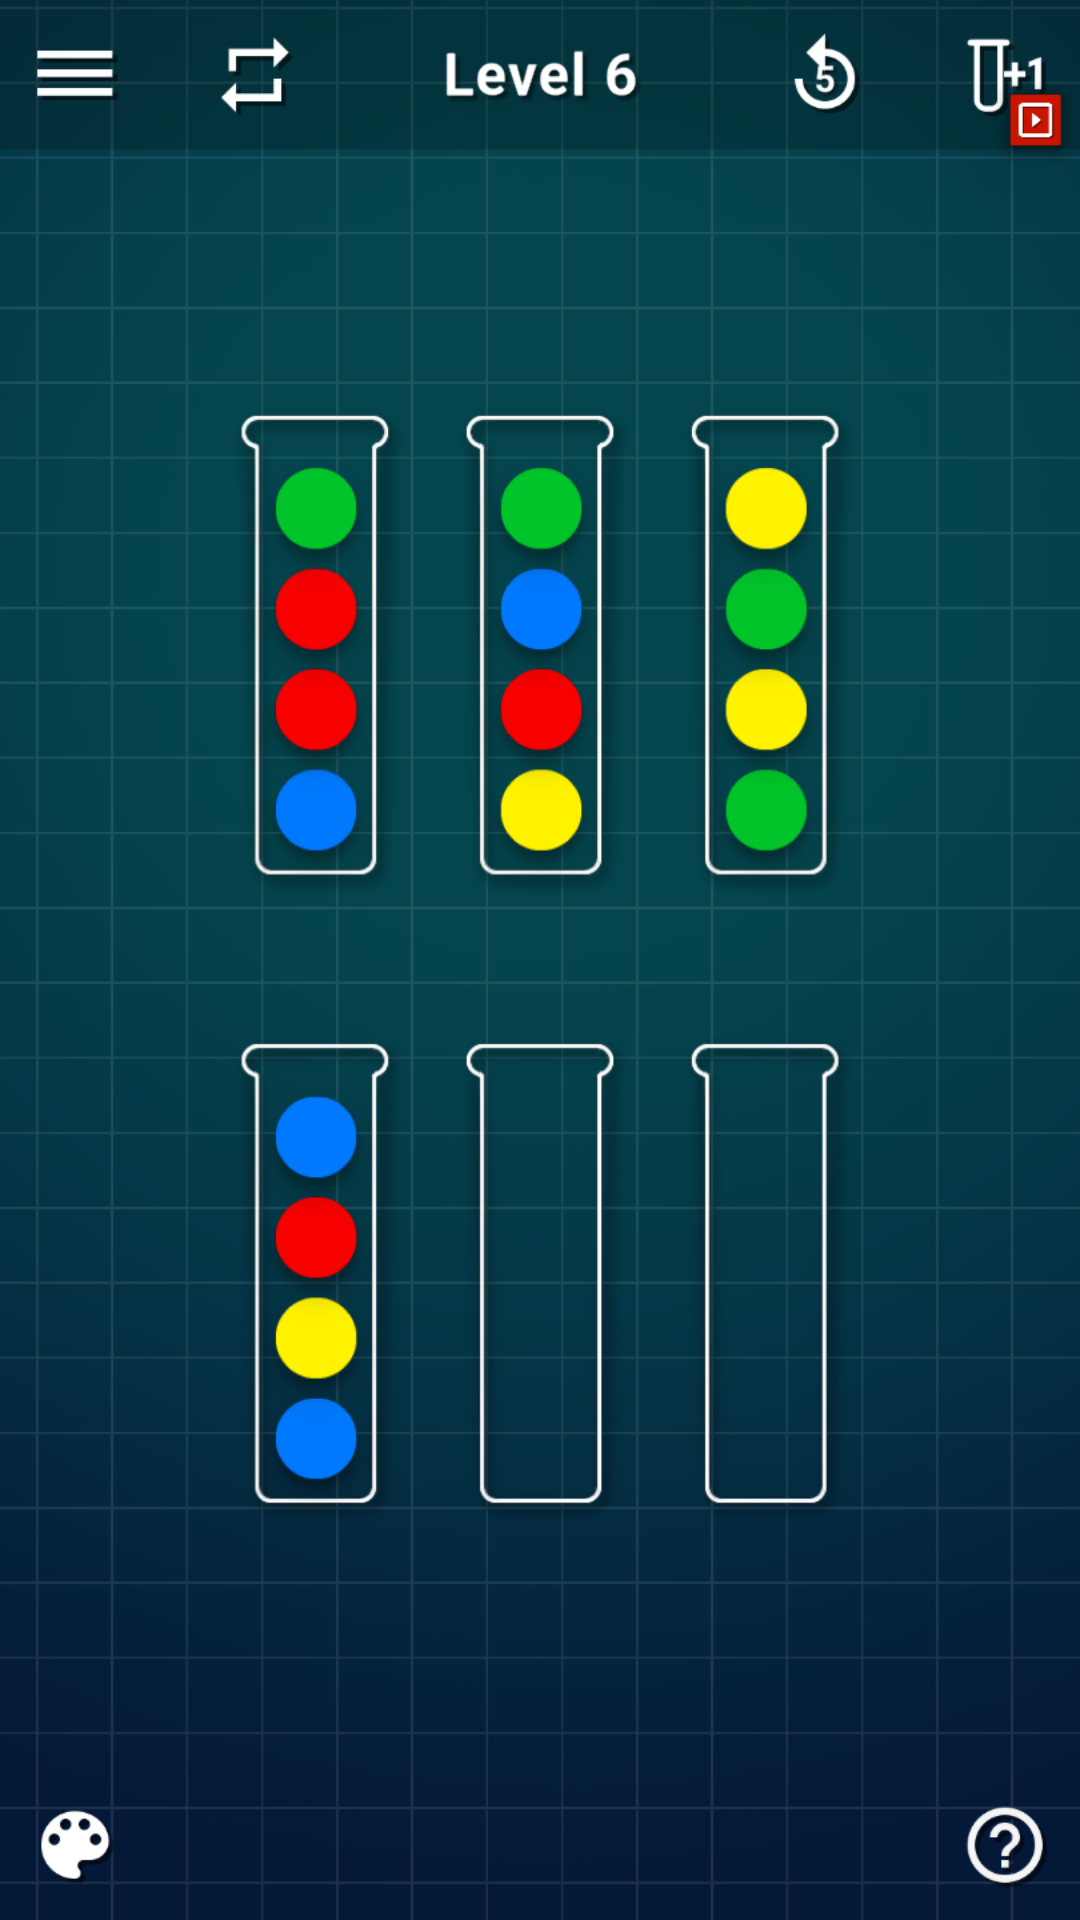
\includegraphics[width=29mm]{img/lvl6-begin.png}
  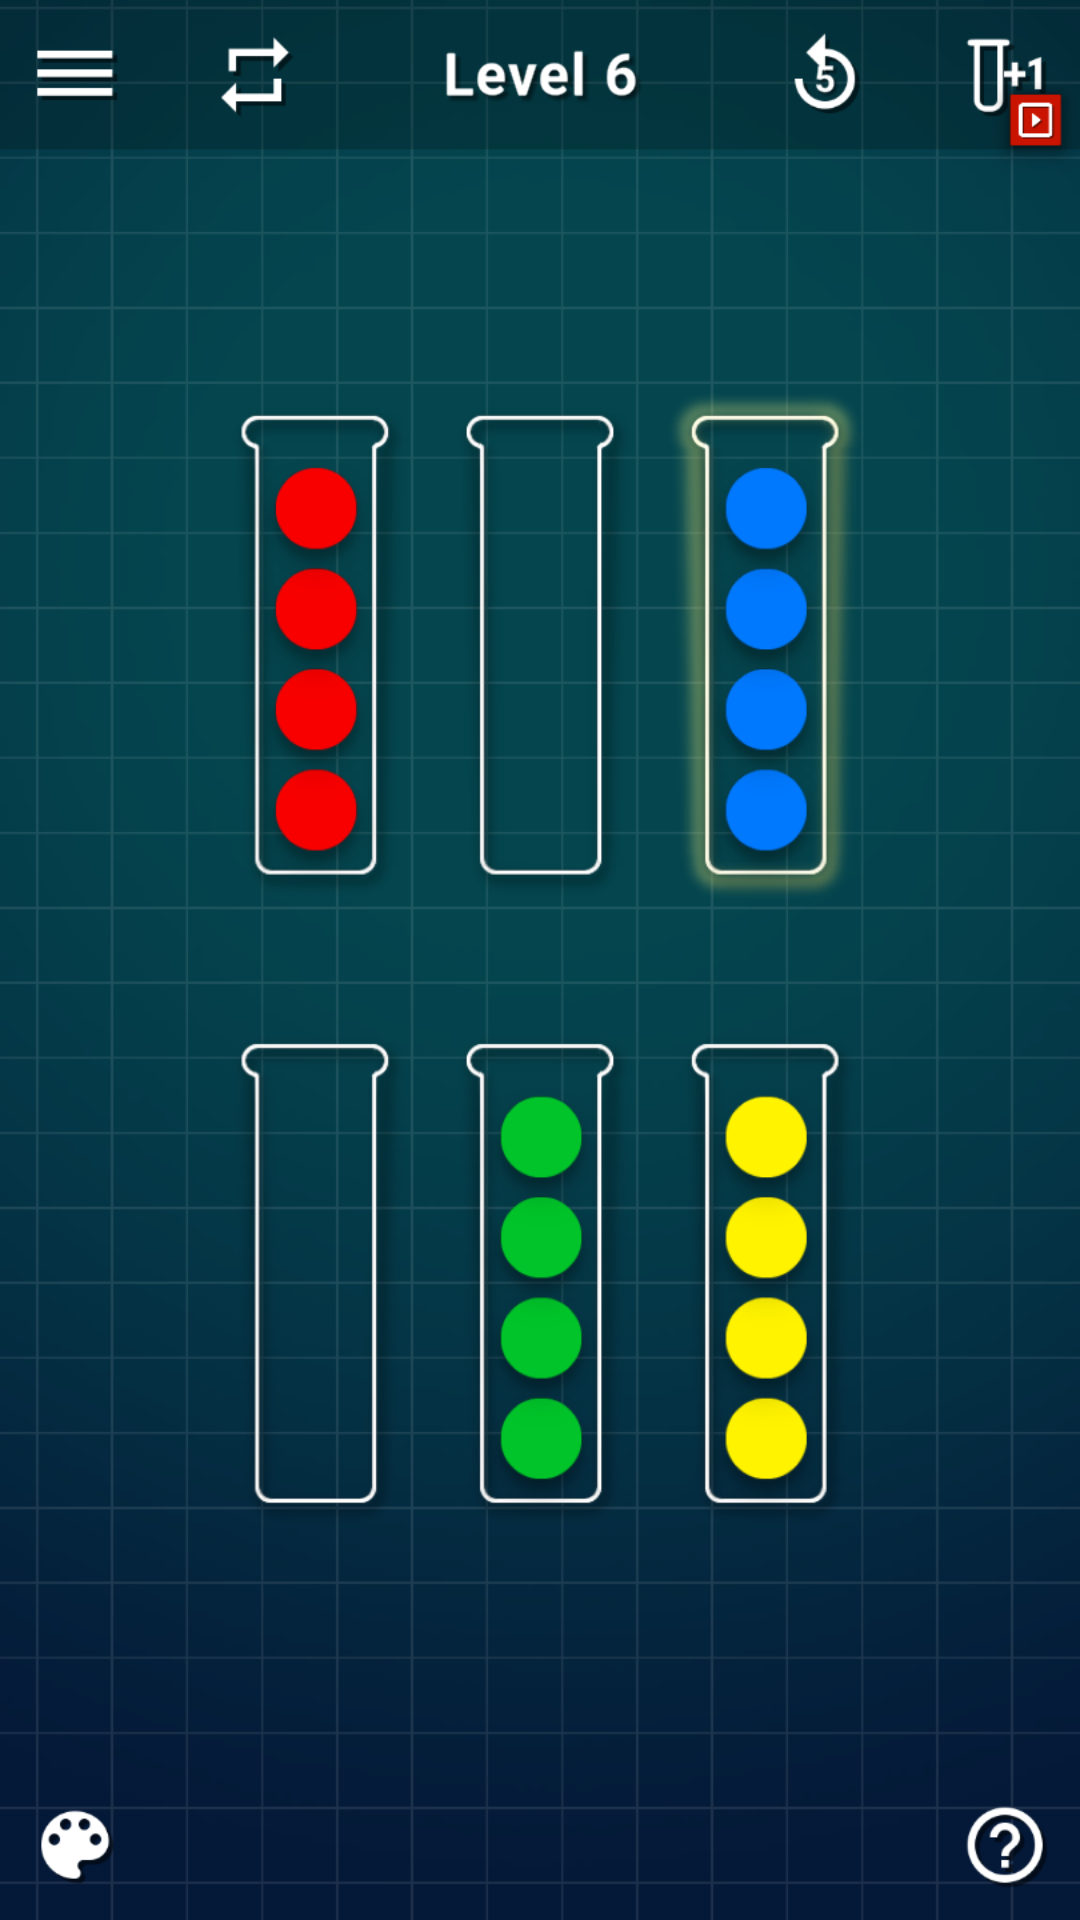
\includegraphics[width=29mm]{img/lvl6-end.png}
\end{minipage}

\end{frame}

\begin{frame}
\frametitle{1. Work specification}
\framesubtitle{1.2. Problem formalization}

\textbf{State} | Vector $S = \langle t_1, t_2, ..., t_N \rangle$ of $N$ tubes with maximum capacity $H$, where tube $i$ is a stack $t_i = \langle t_i(1), t_i(2), ..., t_i(h_i) \rangle$ with $h_i$ balls ($0 \leq h_i \leq H$), where $t_i(1)$ is the color of the ball at the bottom, and $t_i(h_i)$ the color at the top. There are $C$ colors ($C < N$) numbered sequentially, thus $\forall i, j,~1 \leq t_i(j) \leq C$.

\textbf{Action} | The only action is a move $(i,j)$:
\begin{itemize}
  \item Origin \& destination tubes $1 \leq i, j \leq N$ ($i \neq j$).
  \item Pre-conditions: $h_i \geq 1$, $h_j < H$ and either $h_j = 0$ or $t_i(h_i)=t_j(h_j)$.
  \item Post-conditions: $S'$ is built from $S$, except $t_i$ is a ball shorter (say it had color $c$), and $t_j$ has one more ball at the top with color $c$.
\end{itemize}

% \textbf{Policy} | This is what we want to find.

\end{frame}

\begin{frame}

\textbf{Reward} | We first tried the following reward function:

\begin{equation*}
  r = \begin{cases}
    WinReward & \text{if wins} \\
    LoseReward & \text{if loses} \\
    MoveHitReward & \text{if chosen move is valid} \\
    MoveMissReward & \text{if chosen move is invalid}
  \end{cases}
\end{equation*}

Sample values:
\begin{center}
  \footnotesize
  \begin{tabular}{c | c}
    $WinReward = +1$ & $LoseReward=-1$ \\ \hline
    $MoveHitReward = +0.01$ & $MoveMissReward = -0.01$
  \end{tabular}
\end{center}

Then we tried a new reward function \cite{metz2020}:

\begin{equation*}
  r = \begin{cases}
    1 - \frac{1}{4}\frac{nMisses}{MaxMoves} - \frac{1}{4} \frac{nMoves}{MaxMoves} & \text{if wins} \\
    -1 & \text{if loses} \\
    0 & \text{otherwise}
  \end{cases}
\end{equation*}

($MaxMoves = 5000$)

\end{frame}

\begin{frame}
\frametitle{1. Work specification}
\framesubtitle{1.3. Solution description}

\begin{enumerate}
  \itemsep0em
  \item Implement the game
  \item Implement a human-friendly interface.
  \item Use reinforcement learning algorithms (more specifically deep learning) to solve the game and compare performances.
\end{enumerate}

\end{frame}

\begin{frame}
\frametitle{2. Related works}

A few common problems related to stacks, mostly applied to cargo containers.

Assume there is a set of cargo containers in a yard with a certain number of slots, and that containers are stacked to save space.

\vspace{0.5em}

\begin{tabular}{@{}p{46mm} p{70mm}@{}}
  \textbf{Container Pre-Marshalling Problem (CPMP)} & \textbf{Block Relocation Problem (BRP)} \\
  Some containers have more priority than others (e.g., are meant to be shipped first than others), so each stack must be sorted in non-decreasing order of priority from the bottom up with the least number of moves. &
  Containers will be extracted in a specific order (say that the $N$ containers are numbered from $1$ to $N$; container 1 is extracted first, then 2, ..., and finally container $N$). The goal is to extract all containers in that order with the least amount of moves (i.e., if you need to remove container 3 to extract container 1, you'd prefer to put 3 on top of 4 than on top of 2, otherwise you'd have to again relocate 3 to reach 2).
\end{tabular}

\end{frame}

\begin{frame}

\frametitle{2. Related works}
\textbf{Container Pre-Marshalling Problem (CPMP)}

\begin{itemize}
  \item Has been approached before with machine learning:
  \begin{itemize}
    \item \textbf{Reinforcement learning:} Q-learning \cite{hirashima2008}
    \item \textbf{Supervised learning:} \cite{hottung2020} labels nodes using known near-optimal algorithms, and uses a tree search together with deep neural networks (DNN) to select branches and prune the search tree, claims to achieve results 2\% away from optimality.
  \end{itemize}

\end{itemize}

\textbf{Block Relocation Problem (BRP)}

\begin{itemize}
  \item Reinforcement learning has also been applied to BRP; \cite{jiang2021} provides a framework for reinforcement learning on BRP, and applies an heuristic function and $\varepsilon$-greedy strategy.
  % \item Many research has been applied to finding lower bounds, and \cite{zhang2020} presents innovative upper and lower bounds for search tree pruning
  % \item Optimal branch\&bound algorithms with heavy prunning have been applied with decent results for reasonably small instances, which can be improved upon by using a beam search algorithm (basically a best-first search with less memory usage).
\end{itemize}

This research is significant for our problem; even though the problems are quite different in nature, they share some traits with our problem, and can contribute with ideas for our own solutions.

\end{frame}

\begin{frame}
  \frametitle{3. Tools and algorithms}

  \href{https://github.com/Unity-Technologies/ml-agents}{\textbf{ML agents}} | Reinforcement learning
  \begin{itemize}
    \item PPO (Proximal Policy Optimization), on-policy "simple" first-order methods \cite{openai-ppo, schulman2017}
    \item SAC (Soft-Actor Critic), off-policy stochastic policy updating with results that are good and stable over different instances of the same problem \cite{openai-sac, haarnoja2018}
    \item POCA (Parallel Online Continuous Arcing), parallel boosting algorithm \cite{reichler2004}
  \end{itemize}
\end{frame}


\begin{frame}
\frametitle{4. Implementation}

\begin{itemize}
  \item \textbf{Language} | C\#
  \item \textbf{Environment} | Unity engine (v2020.2.2)
\end{itemize}

\textbf{Summary:} game and puzzle generation implemented, human interface implemented, trained PPO, SAC models

\begin{center}
  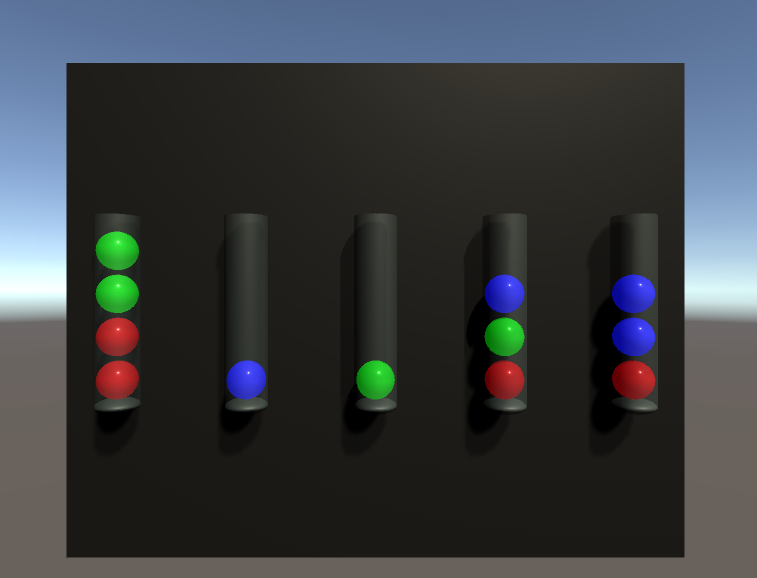
\includegraphics[width=75mm]{img/game-interface.png}
\end{center}

\end{frame}

\begin{frame}
\frametitle{5. Results}

\begin{minipage}[c]{0.45\textwidth}
\begin{center}
  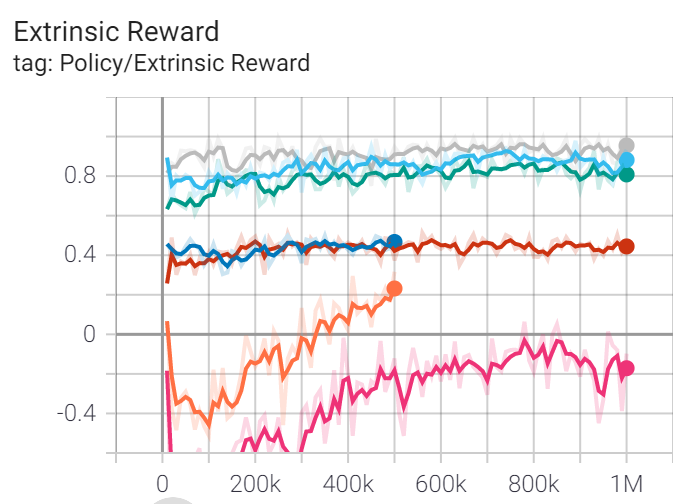
\includegraphics[height=35mm]{img/extrinsic-reward.PNG} \\
  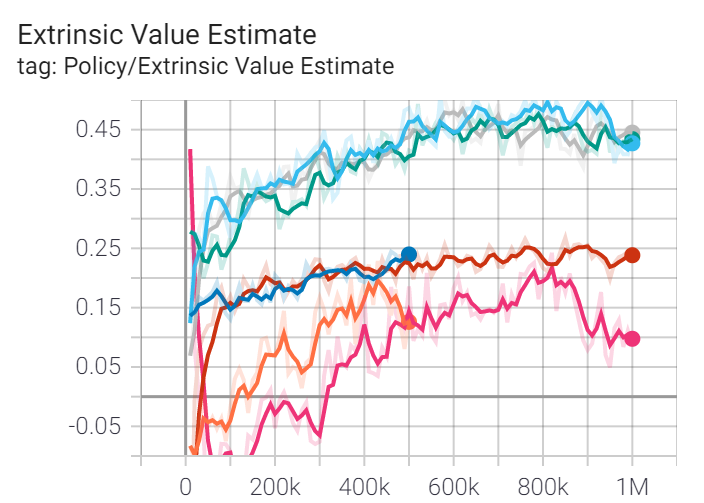
\includegraphics[height=35mm]{img/extrinsic-value-estimate.PNG}
\end{center}
\end{minipage}% 
\begin{minipage}[c]{0.55\textwidth}
\begin{center}
  \small
  \begin{tabular}{l | r r}
    \textbf{Params} & \textbf{Default} & \textbf{Best config} \\ \hline
    batch\_size     & $32$             & $64$                 \\
    buffer\_size    & $10240$          & $2048$               \\
    learning\_rate  & $3\times 10^{-4}$& $3\times 10^{-3}$    \\
    beta            & $5\times 10^{-3}$& $5\times 10^{-2}$    \\
    epsilon         & $0.2$            & $0.5$                \\
    lambd           & $0.95$           & $0.90$               \\
    num\_epoch      & $3$              & $4$                  \\
    gamma           & $0.99$           & $0.995$
  \end{tabular}
\end{center}
\end{minipage}
 

\end{frame}

\begin{frame}
\frametitle{5. Results}
\framesubtitle{5.1. PPO}

Pink | PPO, old reward ~~~~~ Grey | PPO, new reward

\begin{center}
  \begin{tabular}{c c c}
    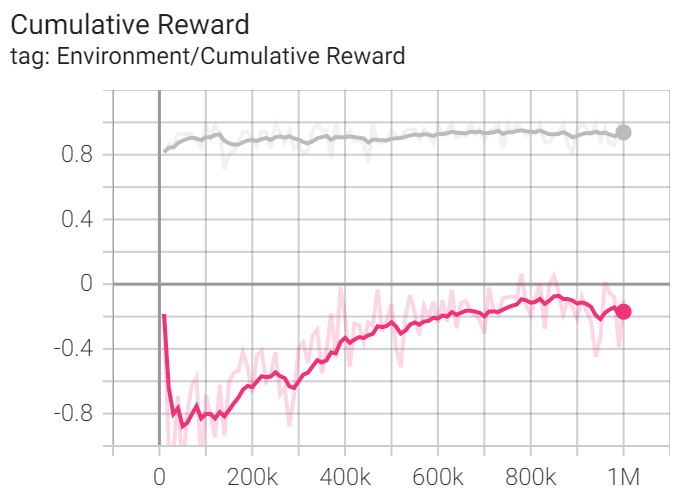
\includegraphics[height=25mm]{img/ppo/ppo-cumulative-reward.PNG} &
    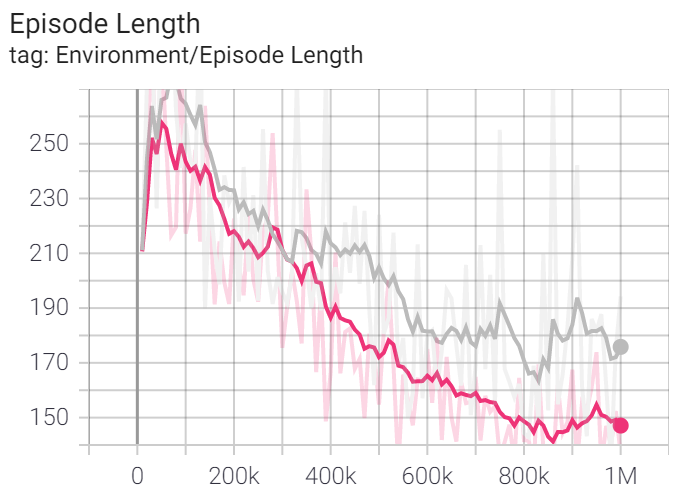
\includegraphics[height=25mm]{img/ppo/ppo-episode-length.PNG} &
    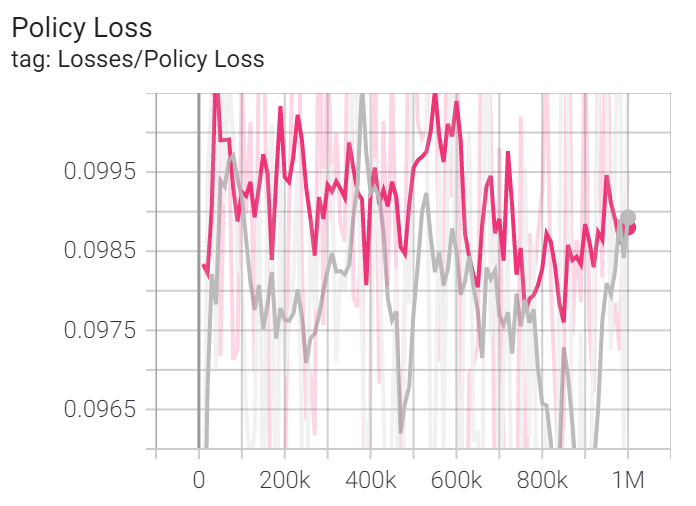
\includegraphics[height=25mm]{img/ppo/ppo-policy-loss.PNG} \\
    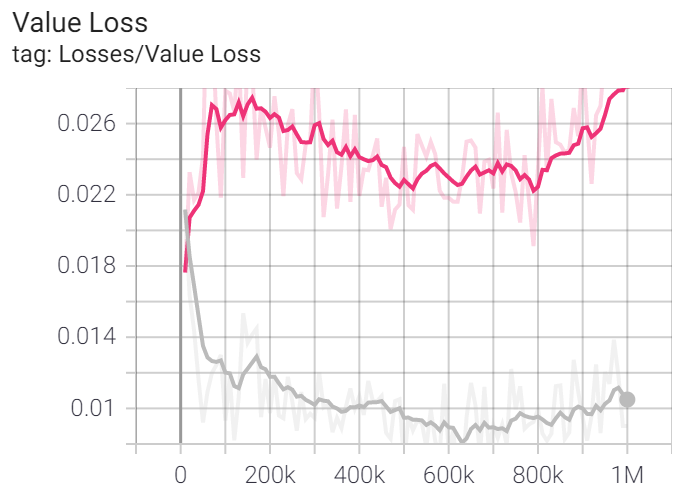
\includegraphics[height=25mm]{img/ppo/ppo-value-loss.PNG} &
    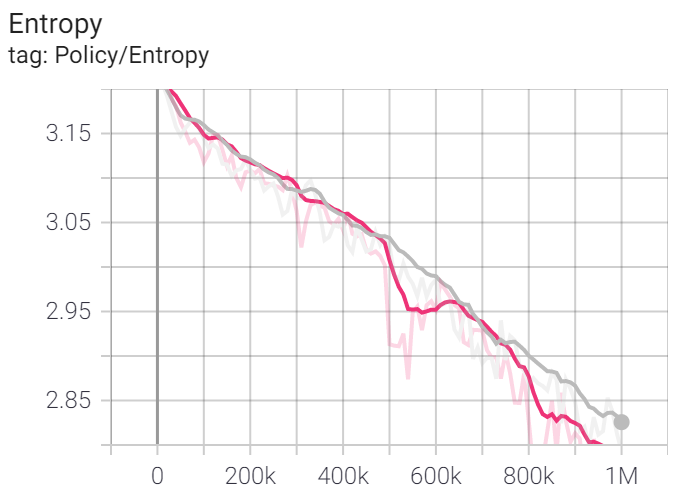
\includegraphics[height=25mm]{img/ppo/ppo-entropy.PNG} &
    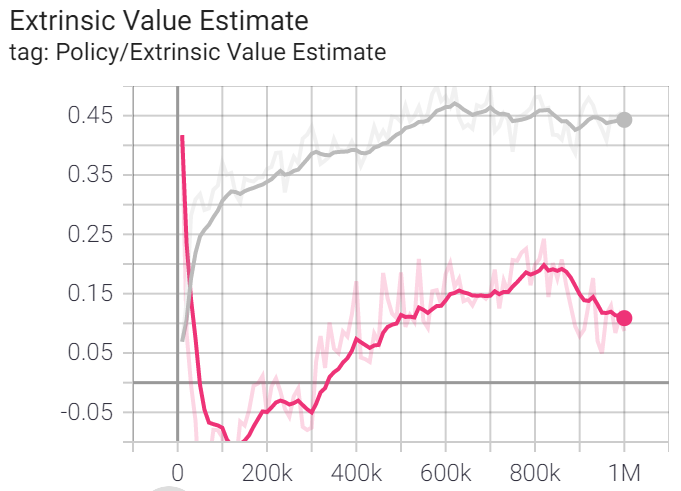
\includegraphics[height=25mm]{img/ppo/ppo-extrinsic-value-estimate.PNG} \\
  \end{tabular}
\end{center}

\begin{center}
  \footnotesize
  \begin{tabular}{l | r | r}
                          & \textbf{Old reward} & \textbf{New reward} \\ \hline
    Success rate (\%)     & $95$                & $95$                \\
    Number of (hit) moves & $24.6$              & $25.0$              \\
    Miss rate (\%)        & $81.9$              & $84.1$              \\
  \end{tabular}
\end{center}

\end{frame}

\begin{frame}
\frametitle{5. Results}
\framesubtitle{5.2. SAC}

Orange | SAC, old reward ~~~~~ Blue | SAC, new reward

\begin{center}
  \begin{tabular}{c c c}
    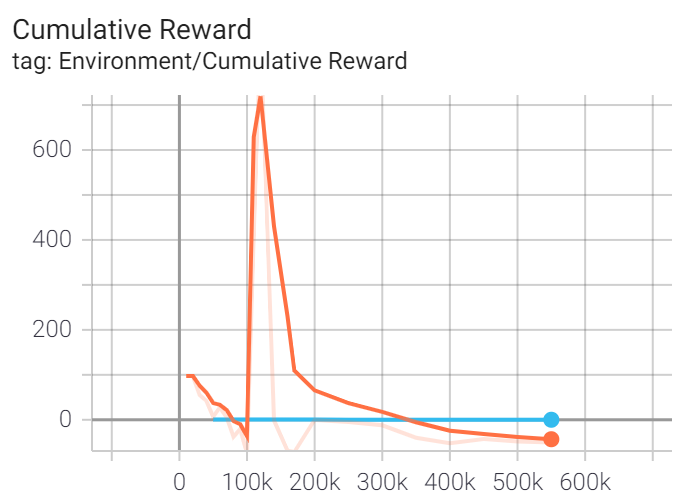
\includegraphics[height=25mm]{img/sac/sac-cumulative-reward.PNG} &
    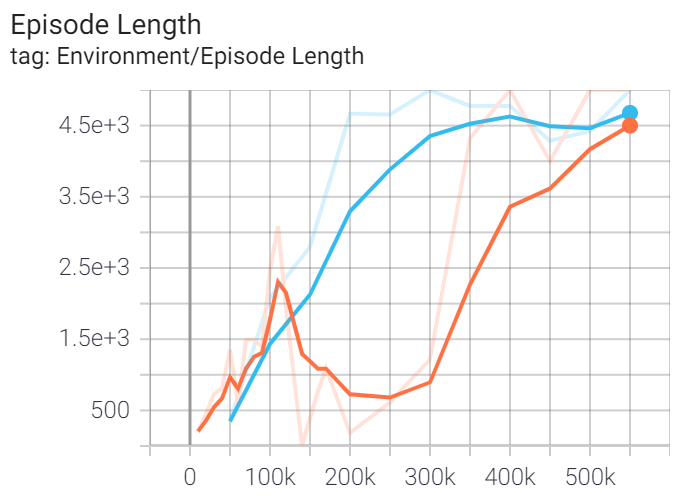
\includegraphics[height=25mm]{img/sac/sac-episode-length.PNG} &
    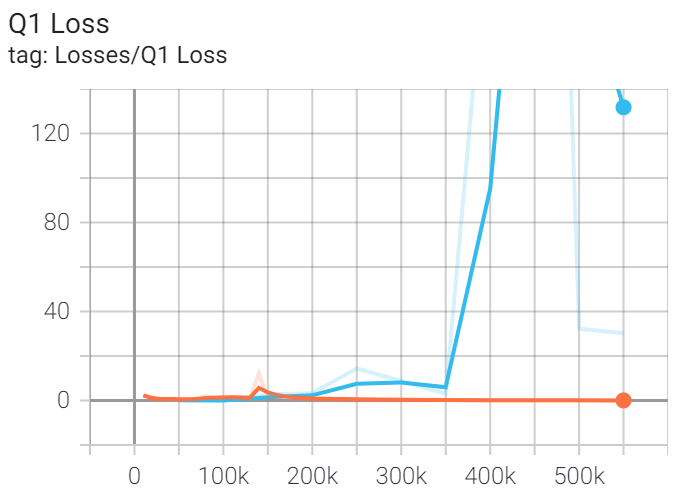
\includegraphics[height=25mm]{img/sac/sac-q1-loss.PNG} \\
    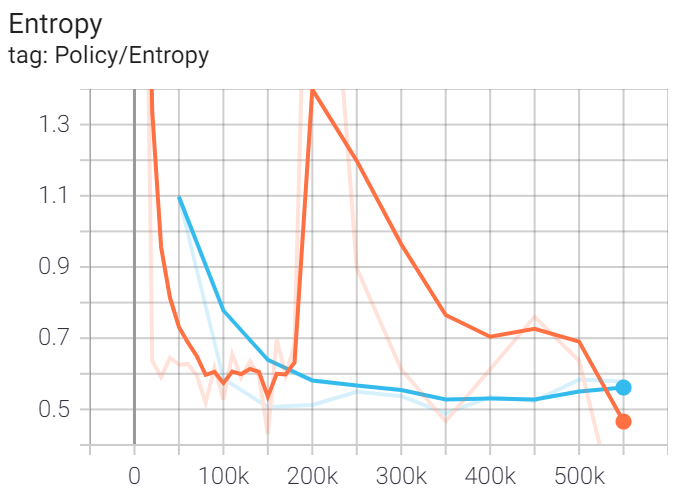
\includegraphics[height=25mm]{img/sac/sac-entropy.PNG} &
    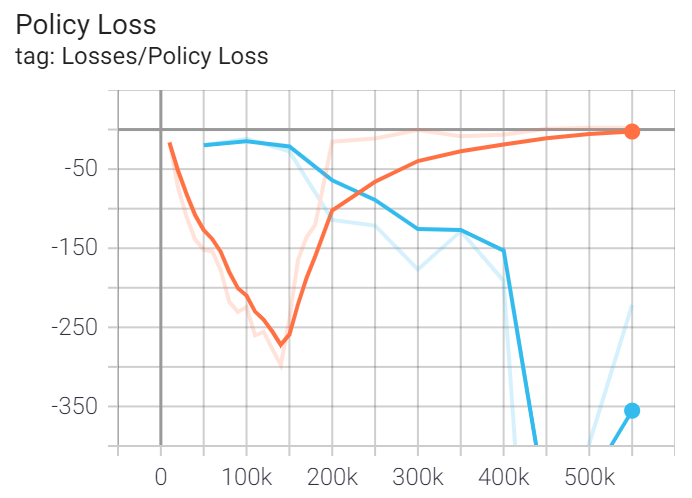
\includegraphics[height=25mm]{img/sac/sac-policy-loss.PNG} &
    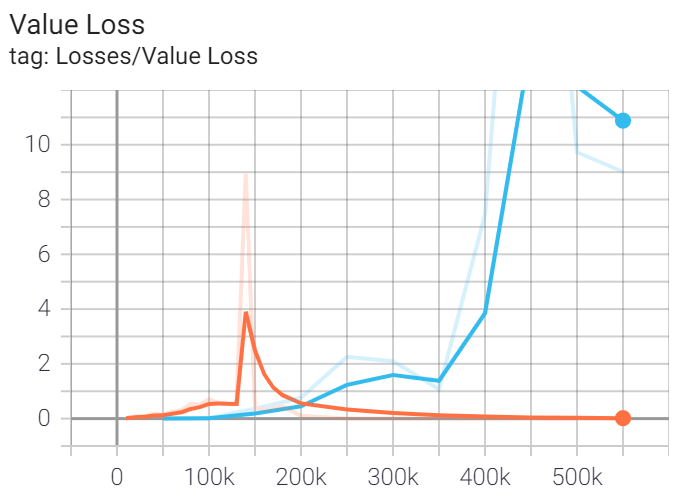
\includegraphics[height=25mm]{img/sac/sac-value-loss.PNG} \\
  \end{tabular}
\end{center}

\begin{center}
  \footnotesize
  \begin{tabular}{l | r | r}
                          & \textbf{Old reward} & \textbf{New reward} \\ \hline
    Success rate (\%)     & $87.5$              & -                   \\
    Number of (hit) moves & $58.85$             & -                   \\
    Miss rate (\%)        & $96.7$              & -                   \\
  \end{tabular}
\end{center}

\end{frame}

\begin{frame}
\frametitle{5. Results}
\framesubtitle{5.3. POCA}

Orange | POCA, old reward ~~~~~ Blue | POCA, new reward

\begin{center}
  \begin{tabular}{c c c}
    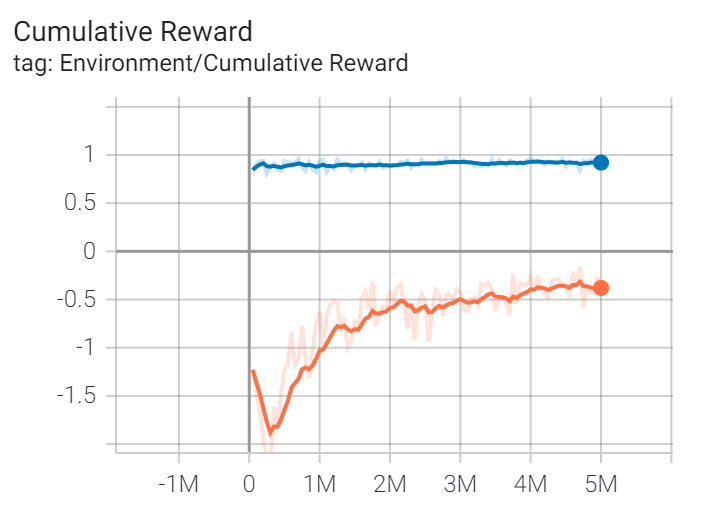
\includegraphics[height=25mm]{img/poca/poca-cumulative-reward.PNG} &
    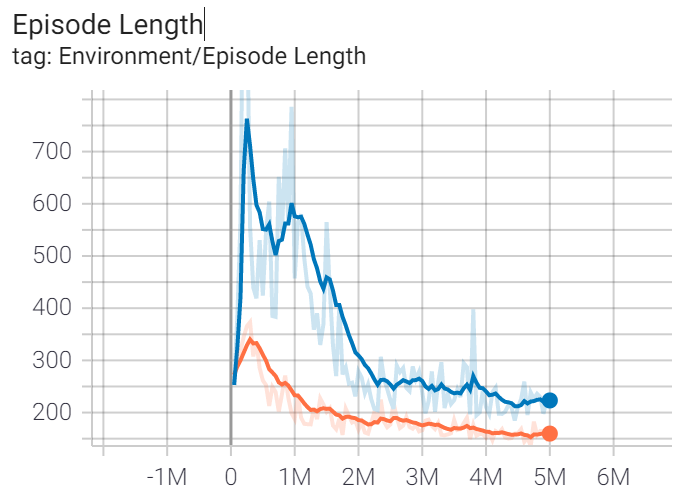
\includegraphics[height=25mm]{img/poca/poca-episode-length.PNG} &
    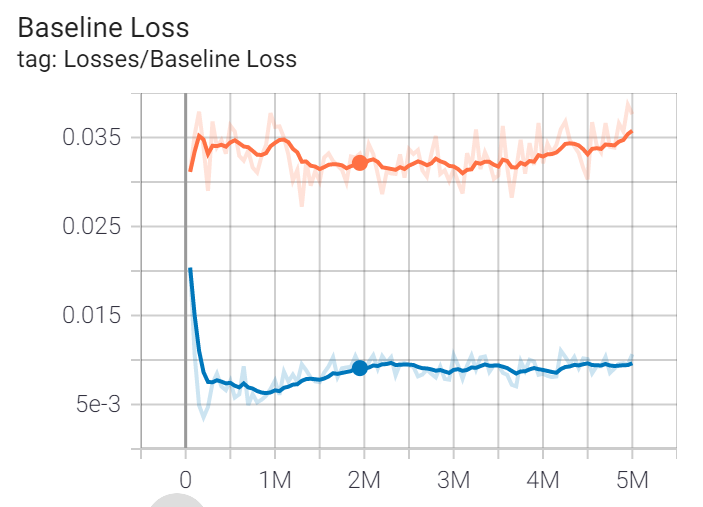
\includegraphics[height=25mm]{img/poca/poca-baseline-loss.PNG} \\
    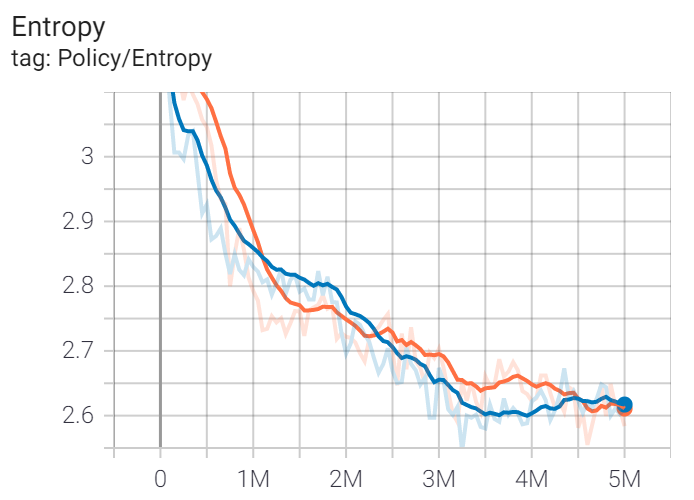
\includegraphics[height=25mm]{img/poca/poca-entropy.PNG} &
    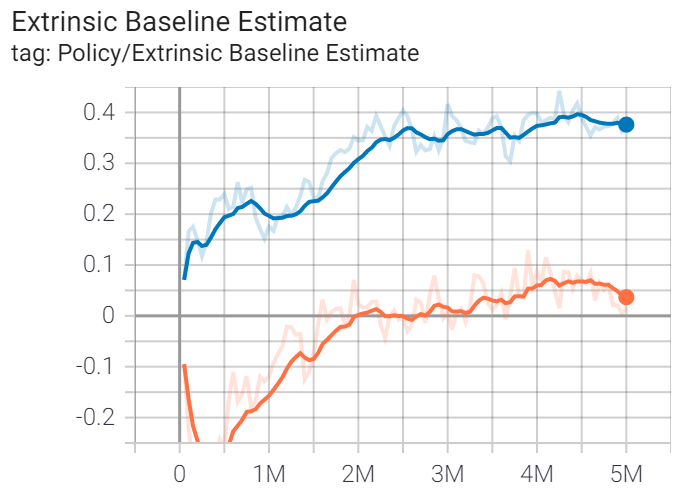
\includegraphics[height=25mm]{img/poca/poca-extrinsic-baseline-estimate.PNG} &
    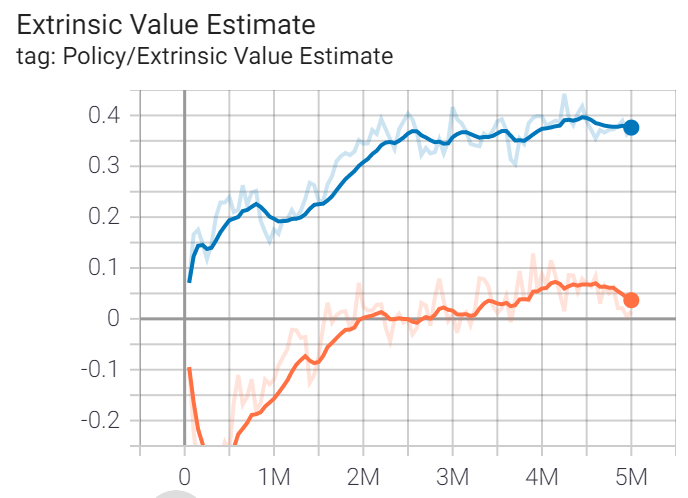
\includegraphics[height=25mm]{img/poca/poca-extrinsic-value-estimate.PNG} \\
  \end{tabular}
\end{center}

\begin{center}
  \footnotesize
  \begin{tabular}{l | r | r}
    \textbf{Best POCA configurations} & \textbf{Old reward} & \textbf{New reward} \\ \hline
    Success rate (\%)                 & $95$                & $97.5$              \\
    Number of (hit) moves             & $20.2$              & $24.9$              \\
    Miss rate (\%)                    & $82.98$             & $85.99$             \\
  \end{tabular}
\end{center}
\end{frame}

\begin{frame}
\frametitle{6. Conclusion}

\begin{itemize}
  \item This puzzle is quite hard for RL.

  \item It was good to simplify the problem to $N=5$, $H=4$, $C=3$, otherwise it would have been even harder. Tested with random puzzles but with same parameters.
  
  \item The two rewards learned in different ways across several algorithms (explicit reward value growth in old formula, good episode time decrease in both), but have similar performance.
  
  \item PPO and POCA learned quite reasonably, SAC yielded poor and inconsistent results and takes a lot of time to train and test. POCA proved slightly better than PPO.
  
\end{itemize}

\end{frame}

\begin{frame}[allowframebreaks]
  \scriptsize
  \frametitle{Bibliography}
  \setbeamertemplate{bibliography item}{\insertbiblabel}
  \bibliographystyle{acm}
  \bibliography{report}
\end{frame}

\end{document}
